\subsection{Held-Out Pixel-Video Results}\label{app:video-results}

Both frozen video evaluations and their artifact audits are complete. Results below use all four model families and persistence on the same cases; this single-training-seed pixel pilot is not a reproduction of the larger latent-space benchmark.

Frame scores average over future leads and weight original source videos equally. FVD uses the selected clip distribution. Time is generation seconds for a complete four-member rollout, and rollout NFE counts neural calls per member over all future frames. Member-FVD SD measures completion randomness, not uncertainty over test cases or training seeds. SI denotes the stochastic interpolant and FM denotes flow matching.

\begin{table*}[t]\centering\small

\begin{tabular}{lrrrrrr}
\toprule
Model & Steps/frame & Rollout NFE & Time (s)$\downarrow$ & CRPS$\downarrow$ & FVD pooled$\downarrow$ & FVD member mean $\pm$ SD \\
\midrule
SI & 16 & 224 & 1.47 & 0.0107 & 436.1 & 485.3 $\pm$ 16.2 \\
SI & 64 & 896 & 5.81 & 0.0094 & 222.3 & 268.9 $\pm$ 10.7 \\
FM & 16 & 224 & 1.45 & 0.0098 & 323.0 & 361.8 $\pm$ 19.1 \\
FM & 64 & 896 & 5.81 & 0.0096 & 330.0 & 372.1 $\pm$ 19.8 \\
It\^o map & 1 & 14 & 0.13 & 0.0140 & 1080.0 & 1117.4 $\pm$ 18.9 \\
It\^o map & 8 & 112 & 0.99 & 0.0110 & 317.3 & 360.5 $\pm$ 6.0 \\
Flow map & 1 & 14 & 0.10 & 0.0110 & 402.2 & 442.7 $\pm$ 5.4 \\
Flow map & 8 & 112 & 0.80 & 0.0101 & 320.4 & 359.9 $\pm$ 15.3 \\
Persistence & 1 & 0 & 0.00 & 0.0107 & 1072.2 & 1071.5 $\pm$ 0.0 \\
\bottomrule
\end{tabular}


\caption{CLEVRER: matched pilot distributional quality and generation cost. Pooled FVD uses 128 real and 512 generated clips; member FVD uses 4 separate 128-versus-128 comparisons. Lower CRPS and FVD are better. Persistence has zero neural evaluations.}\label{tab:video-clevrer-quality}

\end{table*}

\begin{table*}[t]\centering\small

\begin{tabular}{lrrrrrr}
\toprule
Model & Steps/frame & Sample PSNR$\uparrow$ & Sample SSIM$\uparrow$ & Sample LPIPS$\downarrow$ & Mean PSNR$\uparrow$ & Mean SSIM$\uparrow$ \\
\midrule
SI & 16 & 27.34 & 0.803 & 0.174 & 29.05 & 0.864 \\
SI & 64 & 28.47 & 0.876 & 0.141 & 29.63 & 0.884 \\
FM & 16 & 29.32 & 0.883 & 0.136 & 30.10 & 0.892 \\
FM & 64 & 29.19 & 0.879 & 0.140 & 30.06 & 0.888 \\
It\^o map & 1 & 25.69 & 0.601 & 0.283 & 27.79 & 0.785 \\
It\^o map & 8 & 28.00 & 0.860 & 0.148 & 29.21 & 0.880 \\
Flow map & 1 & 28.19 & 0.855 & 0.160 & 29.31 & 0.879 \\
Flow map & 8 & 28.77 & 0.875 & 0.144 & 29.77 & 0.884 \\
Persistence & 1 & 30.05 & 0.904 & 0.127 & 30.05 & 0.904 \\
\bottomrule
\end{tabular}


\caption{CLEVRER: future image quality, averaged across leads. Sample metrics average over completions. Mean PSNR/SSIM score the ensemble-mean image. Image/perceptual metrics use clipped copies; neither feedback nor proper scores are clipped.}\label{tab:video-clevrer-images}

\end{table*}

\begin{table*}[t]\centering\small

\begin{tabular}{lrrrrrrr}
\toprule
Model & Steps/frame & Energy$\downarrow$ & RMSE$\downarrow$ & RMS spread & Spread/skill & Coverage (\%) & Out of range (\%) \\
\midrule
SI & 16 & 0.0283 & 0.0414 & 0.0295 & 0.949 & 73.9 & 0.0 \\
SI & 64 & 0.0288 & 0.0409 & 0.0273 & 0.877 & 55.6 & 0.0 \\
FM & 16 & 0.0302 & 0.0402 & 0.0217 & 0.700 & 47.5 & 0.0 \\
FM & 64 & 0.0296 & 0.0404 & 0.0242 & 0.763 & 45.8 & 0.0 \\
It\^o map & 1 & 0.0300 & 0.0455 & 0.0368 & 1.027 & 77.9 & 0.0 \\
It\^o map & 8 & 0.0303 & 0.0417 & 0.0244 & 0.780 & 65.2 & 0.0 \\
Flow map & 1 & 0.0300 & 0.0412 & 0.0235 & 0.734 & 64.7 & 0.0 \\
Flow map & 8 & 0.0297 & 0.0408 & 0.0249 & 0.781 & 53.8 & 0.0 \\
Persistence & 1 & 0.0428 & 0.0428 & 0.0000 & 0.000 & 80.8 & 0.0 \\
\bottomrule
\end{tabular}


\caption{CLEVRER: additional future-only proper-score and calibration diagnostics. Spread/skill includes the finite-ensemble correction; 90\% denotes the empirical central interval from four members and is not expected to attain 90\% even under ideal calibration. Out-of-range values are measured before display clipping.}\label{tab:video-clevrer-calibration}

\end{table*}

\begin{figure*}[t]\centering

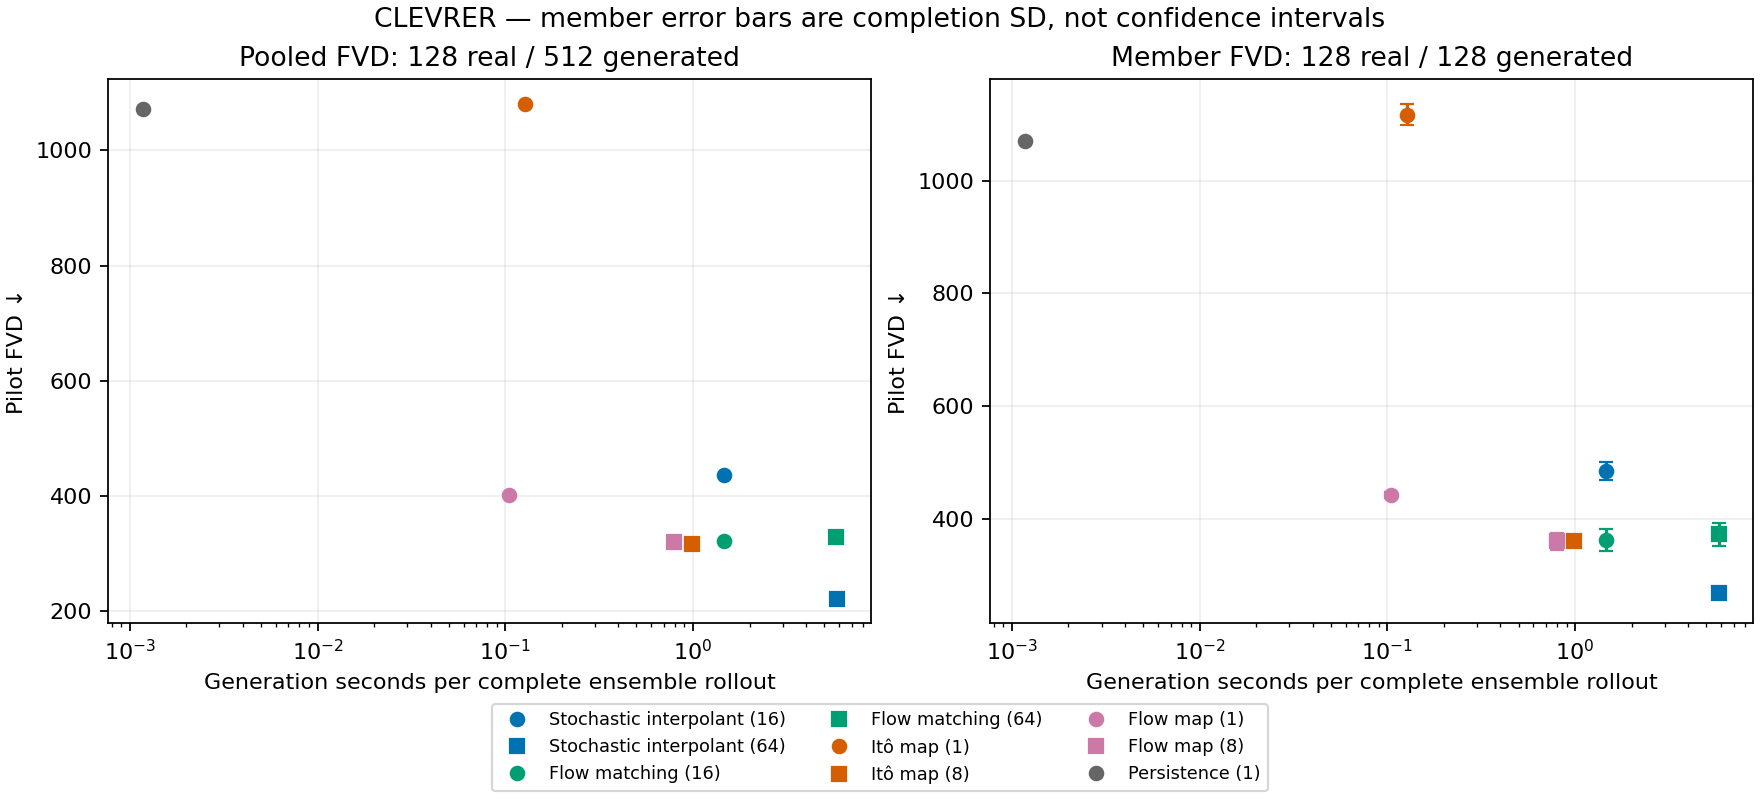
\includegraphics[width=\textwidth]{figures/video_results/clevrer_fvd_vs_cost.png}

\caption{CLEVRER: quality versus complete-ensemble generation cost, copied from the audited report without re-aggregating scores. The right panel uses equal-count member FVD; error bars are completion SD, not confidence intervals.}\label{fig:video-clevrer-cost}

\end{figure*}

\begin{figure*}[t]\centering

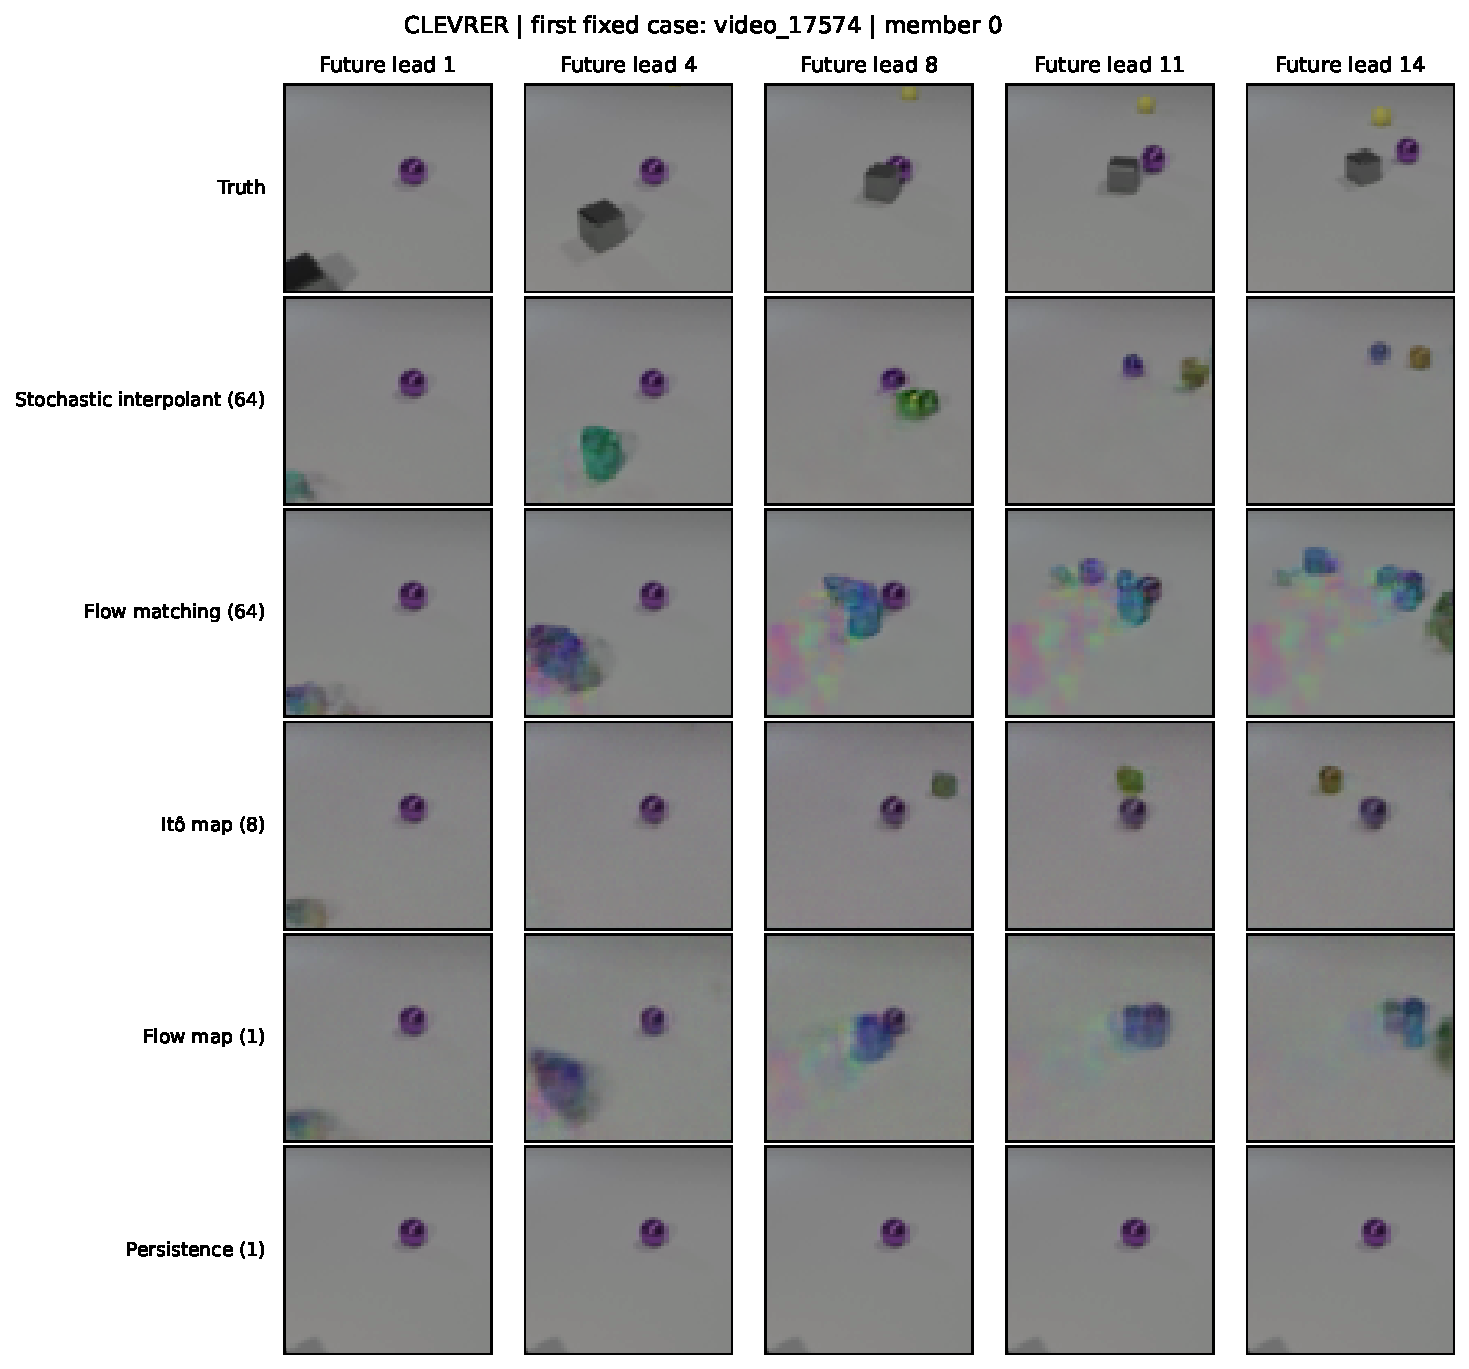
\includegraphics[width=\textwidth,height=.78\textheight,keepaspectratio]{figures/video_results/clevrer_fixed_forecast.pdf}

\caption{CLEVRER: the first preselected test case and ensemble member zero, at fixed future leads. Solver64, It\^o-map8, flow-map1 and persistence budgets were chosen before completed comparisons. All rows share the same observations and truth; no case or member was chosen by forecast quality. Display clips copies to the pixel range.}\label{fig:video-clevrer-forecast}

\end{figure*}

\begin{table*}[t]\centering\small

\begin{tabular}{lrrrrrr}
\toprule
Model & Steps/frame & Rollout NFE & Time (s)$\downarrow$ & CRPS$\downarrow$ & FVD pooled$\downarrow$ & FVD member mean $\pm$ SD \\
\midrule
SI & 16 & 480 & 3.07 & 0.0526 & 1781.7 & 1812.6 $\pm$ 16.3 \\
SI & 64 & 1920 & 12.58 & 0.0285 & 773.5 & 823.0 $\pm$ 20.7 \\
FM & 16 & 480 & 3.12 & 0.0265 & 726.8 & 766.9 $\pm$ 17.2 \\
FM & 64 & 1920 & 12.36 & 0.0264 & 783.1 & 831.5 $\pm$ 21.7 \\
It\^o map & 1 & 30 & 0.28 & 0.0319 & 1271.3 & 1302.2 $\pm$ 18.8 \\
It\^o map & 8 & 240 & 2.07 & 0.0286 & 888.2 & 926.5 $\pm$ 21.1 \\
Flow map & 1 & 30 & 0.23 & 0.0276 & 857.2 & 895.1 $\pm$ 18.1 \\
Flow map & 8 & 240 & 1.67 & 0.0277 & 706.6 & 748.0 $\pm$ 19.0 \\
Persistence & 1 & 0 & 0.00 & 0.0311 & 816.1 & 815.8 $\pm$ 0.0 \\
\bottomrule
\end{tabular}


\caption{KTH: matched pilot distributional quality and generation cost. Pooled FVD uses 128 real and 512 generated clips; member FVD uses 4 separate 128-versus-128 comparisons. Lower CRPS and FVD are better. Persistence has zero neural evaluations.}\label{tab:video-kth-quality}

\end{table*}

\begin{table*}[t]\centering\small

\begin{tabular}{lrrrrrr}
\toprule
Model & Steps/frame & Sample PSNR$\uparrow$ & Sample SSIM$\uparrow$ & Sample LPIPS$\downarrow$ & Mean PSNR$\uparrow$ & Mean SSIM$\uparrow$ \\
\midrule
SI & 16 & 20.55 & 0.480 & 0.377 & 21.46 & 0.626 \\
SI & 64 & 23.74 & 0.735 & 0.171 & 24.87 & 0.779 \\
FM & 16 & 24.30 & 0.769 & 0.163 & 25.25 & 0.790 \\
FM & 64 & 23.72 & 0.749 & 0.165 & 24.92 & 0.777 \\
It\^o map & 1 & 22.25 & 0.486 & 0.349 & 23.73 & 0.660 \\
It\^o map & 8 & 23.42 & 0.706 & 0.193 & 24.56 & 0.755 \\
Flow map & 1 & 24.23 & 0.733 & 0.191 & 25.01 & 0.777 \\
Flow map & 8 & 23.98 & 0.757 & 0.168 & 25.02 & 0.781 \\
Persistence & 1 & 24.77 & 0.805 & 0.165 & 24.77 & 0.805 \\
\bottomrule
\end{tabular}


\caption{KTH: future image quality, averaged across leads. Sample metrics average over completions. Mean PSNR/SSIM score the ensemble-mean image. Image/perceptual metrics use clipped copies; neither feedback nor proper scores are clipped.}\label{tab:video-kth-images}

\end{table*}

\begin{table*}[t]\centering\small

\begin{tabular}{lrrrrrrr}
\toprule
Model & Steps/frame & Energy$\downarrow$ & RMSE$\downarrow$ & RMS spread & Spread/skill & Coverage (\%) & Out of range (\%) \\
\midrule
SI & 16 & 0.0730 & 0.0968 & 0.0452 & 0.612 & 40.3 & 0.0 \\
SI & 64 & 0.0466 & 0.0653 & 0.0380 & 0.717 & 39.2 & 0.0 \\
FM & 16 & 0.0461 & 0.0632 & 0.0348 & 0.662 & 31.4 & 0.2 \\
FM & 64 & 0.0458 & 0.0654 & 0.0415 & 0.760 & 34.2 & 0.2 \\
It\^o map & 1 & 0.0504 & 0.0729 & 0.0483 & 0.828 & 59.1 & 0.2 \\
It\^o map & 8 & 0.0477 & 0.0673 & 0.0410 & 0.714 & 46.5 & 0.3 \\
Flow map & 1 & 0.0481 & 0.0639 & 0.0306 & 0.575 & 41.2 & 0.0 \\
Flow map & 8 & 0.0467 & 0.0648 & 0.0376 & 0.691 & 31.8 & 0.3 \\
Persistence & 1 & 0.0674 & 0.0674 & 0.0000 & 0.000 & 18.7 & 0.0 \\
\bottomrule
\end{tabular}


\caption{KTH: additional future-only proper-score and calibration diagnostics. Spread/skill includes the finite-ensemble correction; 90\% denotes the empirical central interval from four members and is not expected to attain 90\% even under ideal calibration. Out-of-range values are measured before display clipping.}\label{tab:video-kth-calibration}

\end{table*}

\begin{figure*}[t]\centering

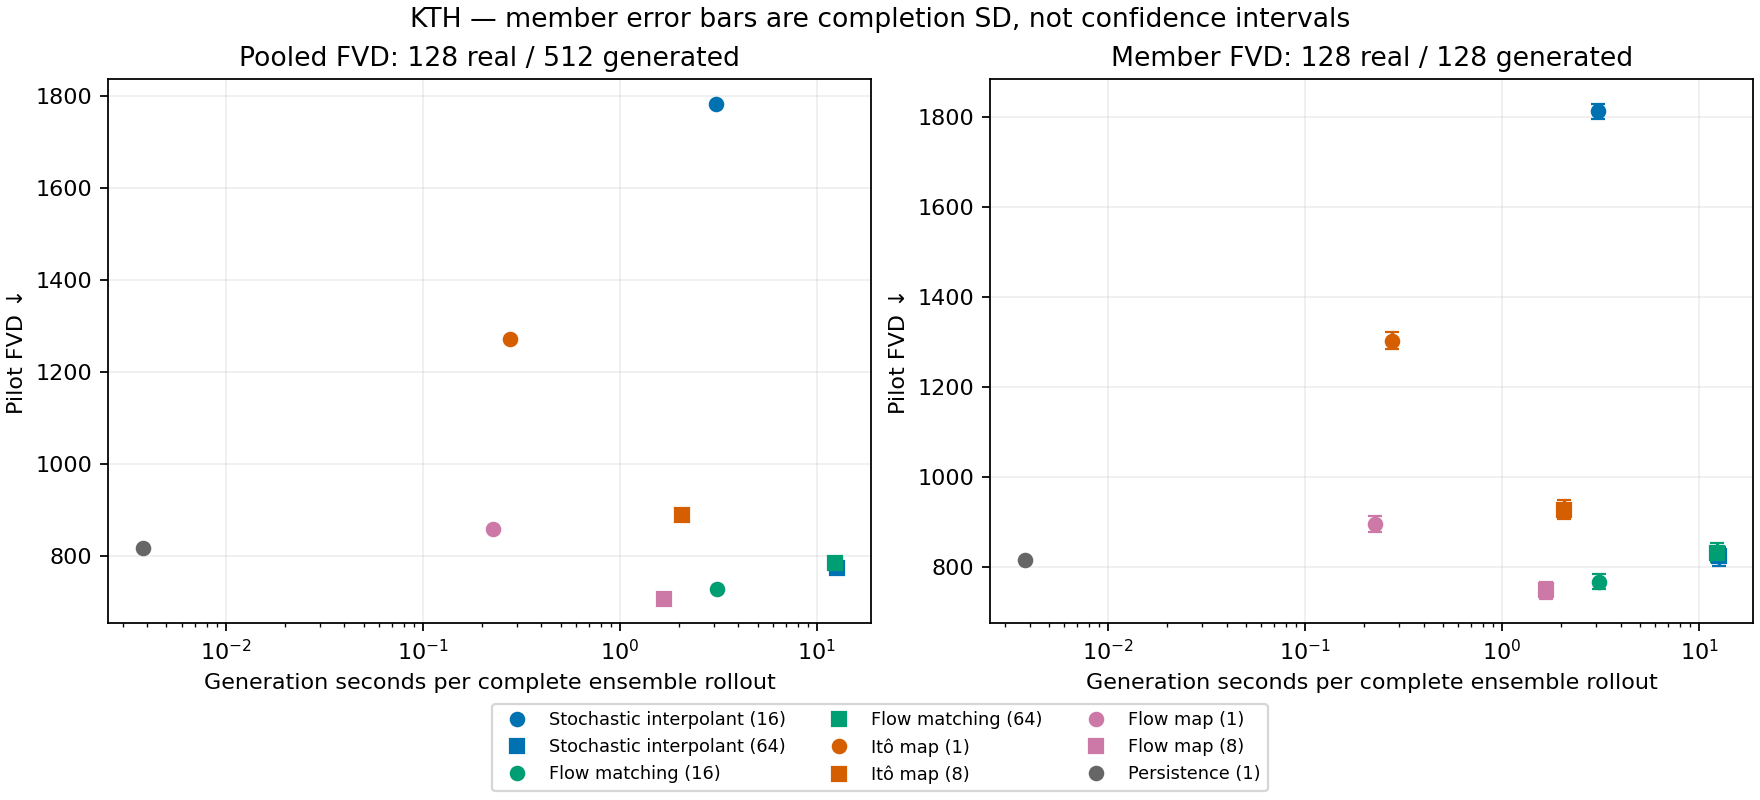
\includegraphics[width=\textwidth]{figures/video_results/kth_fvd_vs_cost.png}

\caption{KTH: quality versus complete-ensemble generation cost, copied from the audited report without re-aggregating scores. The right panel uses equal-count member FVD; error bars are completion SD, not confidence intervals.}\label{fig:video-kth-cost}

\end{figure*}

\begin{figure*}[t]\centering

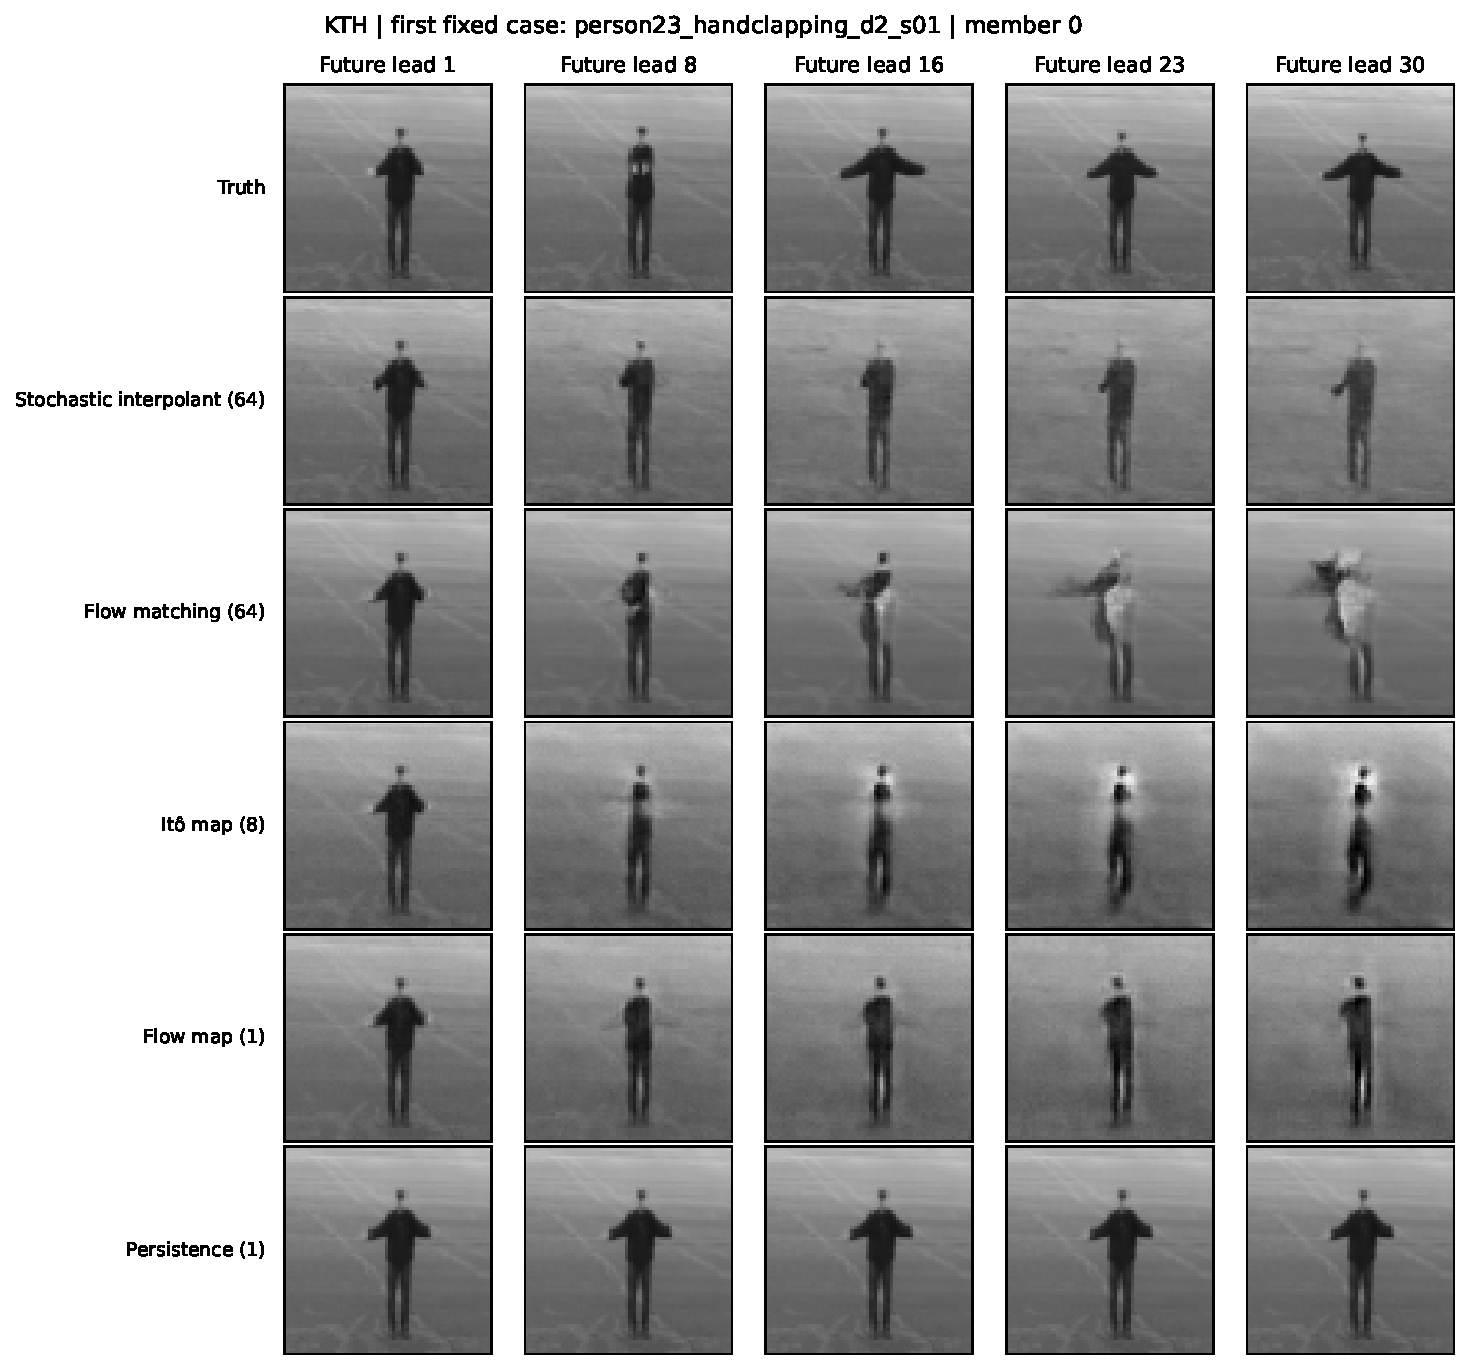
\includegraphics[width=\textwidth,height=.78\textheight,keepaspectratio]{figures/video_results/kth_fixed_forecast.pdf}

\caption{KTH: the first preselected test case and ensemble member zero, at fixed future leads. Solver64, It\^o-map8, flow-map1 and persistence budgets were chosen before completed comparisons. All rows share the same observations and truth; no case or member was chosen by forecast quality. Display clips copies to the pixel range.}\label{fig:video-kth-forecast}

\end{figure*}

Full per-lead source-video bootstrap intervals, additional oracle-member metrics and the unrounded aggregate metrics remain in the accompanying machine-readable reports. These intervals do not quantify training-seed variation. The finite-member forecast examples are illustrative rather than evidence of calibrated conditional uncertainty.
